\subsection{平展映射的连续提升}

设 \(p \colon \mathrm{E} \to \mathrm{B}\) 与 \(f \colon \mathrm{Z} \to \mathrm{B}\) 为连续映射。\(f\) 到 \(\mathrm{E}\) 中的一个连续提升是指一个连续映射 \(g \colon \mathrm{Z} \to \mathrm{E}\) ，使得 \(p \circ g = f\) 。\(f\) 到 \(\mathrm{E}\) 中的连续提升所成的集合不是别的，正是 \(\mathcal{C}_{\mathrm{B}}(\mathrm{Z};\mathrm{E})\) 。它也可以等同于集合 \(\mathcal{S}(\mathrm{Z};\mathrm{Z} \times_{\mathrm{B}}\mathrm{E})\) ，即 Z-空间 \((\mathrm{Z} \times_{\mathrm{B}}\mathrm{E},\mathrm{pr}_{1})\) 的投影的连续截面所成的集合。

若 T 是 Z 的一个子集，则 f 到 E 中的一个在 T 上定义的连续提升称为 f \textbar{} T 到 E 中的一个连续提升：

\pandocbounded{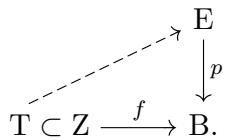
\includegraphics[keepaspectratio]{images/part001_46887bc2.jpg}}

命题 10. --- 设 E、B 与 Z 为拓扑空间，\(p\colon E \to B\) 为一个平展映射，\(f\colon Z \to B\) 为一个连续映射。

设 \(z \in \mathbf{Z}\) 与 \(x \in \mathrm{E}\) 为满足 \(f(z) = p(x)\) 的点。存在一个邻域 \(\mathrm{W}\) （\(z\) 的，在 \(\mathbf{Z}\) 上），以及一个连续提升 \(g\) （\(f\) 的，到 \(\mathrm{E}\) 中），它在 \(\mathrm{W}\) 上定义且满足 \(g(z) = x\) 。

存在 \(p(x)\) 在 B 中的一个开邻域 V 以及 p 在 V 上的一个连续截面 s，使得 \(s(p(x)) = x\) (命题 9)。集合 \(W = f^{-1}(V)\) 是 z 的一个开邻域，而映射 \(g = s \circ (f|W)\) 是 f 到 E 中的一个连续提升，它在 W 上定义且满足 \(g(z) = x\) 。

命题 11. --- 设 E、B 与 Z 为拓扑空间，\(p\colon E \to B\) 与 \(f\colon Z \to B\) 为连续映射。设 \(g\) 与 \(g'\) 为 \(f\) 到 E 中的连续提升。设 W 为 Z 中使 \(g\) 与 \(g'\) 相等的点所成的集合。

\begin{enumerate}
\def\labelenumi{\alph{enumi})}
\item
  若映射 p 是分离的，则 W 是闭的。
\item
  若映射 p 是平展的，则 W 是开的。
\end{enumerate}

用 \(h\) 表示连续映射 \((g, g')\colon Z \to E \times E\) 。\(h\) 的像包含于 \(E \times_{B} E\) 中，因为 \(p \circ g = f = p \circ g'\) ，而 Z 中使 g 与 g' 相等的点所成的集合 W，就是 \(h\) 之下对角线 \(\Delta_{E}\) 的原像。

若映射 p 是平展的，则对角线 \(\Delta_{E}\) 在 \(E \times_{B} E\) 中是开的 (I, p. 31, prop. 7)，从而集合 W 在 Z 中是开的。

若映射 p 是分离的，则对角线 \(\Delta_{E}\) 在 \(E \times_{B} E\) 中是闭的 (I, p. 25, def. 1)，从而集合 W 在 Z 中是闭的。

推论 1. --- 若空间 Z 是连通的且映射 p 是平展且分离的，则在某一点相等的 f 到 E 中的连续提升都相等。

推论 2. --- 设 \(p\colon E \to B\) 为一个分离的平展映射。若空间 E 是连通的，则群 \(\mathrm{Aut}_{\mathrm{B}}(\mathrm{E})\) 自由地作用在 E 上。

事实上，若 \(f: \mathrm{E} \to \mathrm{E}\) 是一个 B-态射，则由推论 1，f 与 \(\mathrm{Id}_{\mathrm{E}}\) 相等的点所成的集合是 E 或空集。

推论 3. --- 设 E、B 与 Z 为拓扑空间，\(p\colon E \to B\) 为一个分离的平展态射，\(f\colon Z \to B\) 为一个连续映射。对 \(i = 1,2\) ，设 \(U_i\) 为 Z 的一个开（相应地，闭）子集，\(g_i\colon U_i \to E\) 为 f 的一个在 \(U_i\) 上定义的连续提升。假设交 \(U_1 \cap U_2\) 是连通的，且存在 \(U_1 \cap U_2\) 的一个点 z，使得 \(g_1(z) = g_2(z)\) 。则存在 f 的一个在 \(U_1 \cup U_2\) 上定义的连续提升，它是 \(g_1\) 与 \(g_2\) 的延拓。

由推论 1，在 \(U_{1} \cap U_{2}\) 上，\(g_{1}\) 与 \(g_{2}\) 的限制相等。映射 \(g: U_{1} \cup U_{2} \to E\) ——由 \(g(z) = g_{i}(z)\) （对 \(z \in U_{i}\) ，i = 1, 2）定义——是 f 的一个在 \(U_{1} \cup U_{2}\) 上定义的连续提升 (TG, I, p. 19, prop. 4)。

在前面的结果中，Z = B 且 \(f = Id_{B}\) 的特殊情形是重要的：这时 f 的连续提升就是 p 的连续截面。

命题 12. --- 设 \(p \colon E \to B\) 为一个平展映射。为使映射 \(p\) 是分离的，必须且只需：对每个开子集 \(V\) （\(B\) 的）与每对 \((s, s')\) （\(p\) 在 \(V\) 上的连续截面的对），使 \(s\) 与 \(s'\) 相等的点所成的集合在 \(V\) 中是闭的。

该条件是必要的 (命题 11, I, p. 34)。我们来证明它是充分的。设 \(b\) 为 B 的一个点，并设 \(x\) 与 \(x'\) 为 E 的两个不同的点，满足 \(p(x) = p(x') = b\) 。设 V 为 b 的一个开邻域，s 与 s' 为 p 在 V 上的连续截面，使得 \(s(\mathrm{V})\) 与 \(s'(\mathrm{V})\) 分别是 x 与 x' 的开邻域 (命题 9)。按假设，由点 \(x \in \mathrm{V}\) （满足 \(s(x) \ne s'(x)\) ）组成的集合 W 在 V 中是开的，从而在 B 中也是开的。集合 \(s(\mathrm{W})\) 与 \(s'(\mathrm{W})\) 分别是 x 与 x' 的开邻域；它们按构造是不相交的。这就证明了映射 p 是分离的 (I, p. 25, 定义 1)。
% semantic-fragments: legacy-input-seam
\relax{}
